%!TEX root = ../../main.tex


\begin{figure}[!htb]
\centering
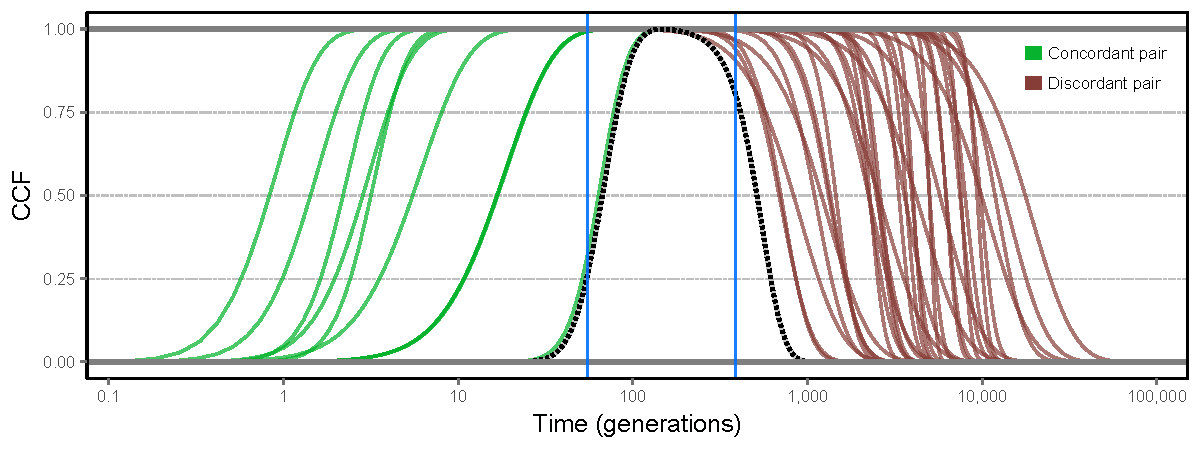
\includegraphics[width=\textwidth]{./img/ch5/age_example_new}
\Caption{Example of concordant and discordant posterior distributions and the resulting composite posterior}%
{A target variant was randomly selected from simulated data.
The \gls{ccf} was obtained for the set of possible concordant pairs and a random subset of discordant pairs.
The thicker \emph{dotted} line shows the distribution of the maximised composite posterior.
The \emph{blue} lines mark the actual time of coalescent events below and above the focal mutation event; \ie $t_c$ (\emph{left}) and $t_d$ (\emph{right}), determined from simulation records.
Their distance corresponds to the length of the branch on which the focal mutation event occurred.}%
{fig:age_example}
\end{figure}
